\documentclass[preprint,12pt]{elsarticle}
\usepackage{amsmath,amssymb,amsfonts}
\usepackage{graphicx}
\usepackage{booktabs}
\usepackage{multirow}
\usepackage[colorlinks=true,allcolors=blue]{hyperref}
\usepackage{xcolor}
\journal{Robotics and Autonomous Systems}
\begin{document}
\begin{frontmatter}
\title{Compliance by Construction:\\ A Quantile-Certified Return-Cost Constraint\\ for Energy-Budgeted Reach Maximization in NMPC}
\author[1]{Nischal Dhakal}
\ead{l202520011@stu.cqupt.edu.cn}
\affiliation[1]{organization={School of Automation, Chongqing University of Posts and Telecommunications}, city={Chongqing}, postcode={400065}, country={China}}
\author[2]{Shuaiyong Li\corref{cor1}}
\ead{lishuaiyong@cqupt.edu.cn}
\affiliation[2]{organization={Key Laboratory of Industrial Internet of Things and Networked Control, Ministry of Education, Chongqing University of Posts and Telecommunications}, city={Chongqing}, postcode={400065}, country={China}}
\cortext[cor1]{Corresponding author.}
\begin{abstract}
A mobile robot on a finite battery must travel as far as its mission
requires and still return. We formulate maximum-reach out-and-back
operation as mission-length nonlinear model predictive control (NMPC)
with a hard terminal reserve constraint,
$E_N + a_q + D_J(x_N) \le B$, where $D_J$ is a terrain-weighted
energy-to-dock geodesic field and $a_q$ is a per-map intercept
certified as the 95th percentile of a fallback policy's realized excess
return cost --- a coverage construction, not a regression fit. Across
2{,}070 missions on nine generated maps under nominal, held-out, and
$\pm 15\%$ plant/model-mismatch regimes, the constrained arm records
zero hard-budget breaches in 480 missions while priced-heuristic NMPC
arms breach 92 of 960 (two-sided Fisher $p = 1.8\times10^{-17}$). The
same certificate tightening that raises the estimators' breach counts
(priced arms $73\to92$ of 960; a plan-then-track oracle
$11\to53$ of 360) leaves the constrained arms at zero: the
certificate's error is absorbed by feasibility, not by the accuracy of
the return policy. The constrained arm realises 64.5\% of the oracle's
reach; the gap is dominated by early turn-backs, an engineering target
rather than a property of the constraint. The certificate's
conservatism is a measured dial: refitting the fallback's terrain speed
shrinks intercepts by 29\% on average at unchanged coverage, buying
$+0.63$ m of reach (Wilcoxon $p = 2.8\times10^{-7}$) at zero breaches.
All results are simulation; the certificate is a rollout-level coverage
bound rather than an invariance barrier, and both limits are quantified.
\end{abstract}

\begin{keyword}
Model predictive control \sep energy-aware robotics \sep mobile robots \sep constrained control \sep persistent autonomy \sep energy management.
\end{keyword}

\end{frontmatter}

\section{Introduction}
% truth_paper.md §1. Framing: energy allocation and reserve, not
% depletion. The law: a hard terminal constraint on a state-dependent
% return-cost estimate ENFORCES budget compliance where fixed prices
% only ENCOURAGE it.
Mobile robots on battery power increasingly run
missions whose value is measured at the far end of a round trip:
inspect as far as the corridor reaches, then come back; sense as many
stations as possible, then return to the dock. We call this mission
class \emph{energy-budgeted reach maximization}: depart from the dock,
travel as far as the mission requires, and return before the pack is
exhausted. The class covers persistent-autonomy sensing rounds,
inspection patrols, and any out-and-back excursion whose success is
conditional on coming home \cite{notomista2021persistification,
huang2015adaptive}. The budget $B$ is hard in the physical sense: a
mission that returns with a negative balance has failed in a way no
score can repair.

The controlling physics is unforgiving. For the differential-drive
platform studied here, specific energy
$\lambda(v) = P(v)/v$ of the drive train is a convex function of speed
with an analytic floor $\lambda_{\min} = 2\sqrt{c_1 c_5} + c_4 =
6.68$~J/m at the energy-minimising cruise speed $v^{*} = 1.10$~m/s
% <- truth §1 (λ_min = 6.677226 J/m, v* = 1.095445 m/s; c adopted)
(Section~\ref{sec:formulation}). Over the cruise band
$v \in [1.0, 1.2]$~m/s the floor varies by 0.34\%
($6.677 \le \lambda \le 6.700$~J/m): there is no meaningful speed lever
on energy. The one lever the robot controls is \emph{where it turns
around} --- and that decision depends on a quantity it cannot measure
directly: the energy the return leg will actually cost.

The field's dominant practice prices that decision with a hand-tuned
margin: drive the outbound leg, and turn back when the remaining
energy falls below $\gamma$ times the estimated cost-to-home, with
$\gamma$ chosen by the operator's experience
\cite{huang2015adaptive, li2026robust}. The margin is real, but its
size is calibration: too small and the robot strands mid-return, too
large and it throws away reach it could have spent. Compliance under
such policies is a property of the tuning session, not of the control
law. The alternative we study is to make the margin an input to a hard
constraint inside the NMPC: at the end of every planned horizon the
predicted pack state plus a certified return reserve must fit inside
the budget. A hard constraint enforces what a penalty merely
encourages; the engineering question is what the reserve should be,
and that question has a data-driven answer.

\begin{figure*}[!t]
\centering
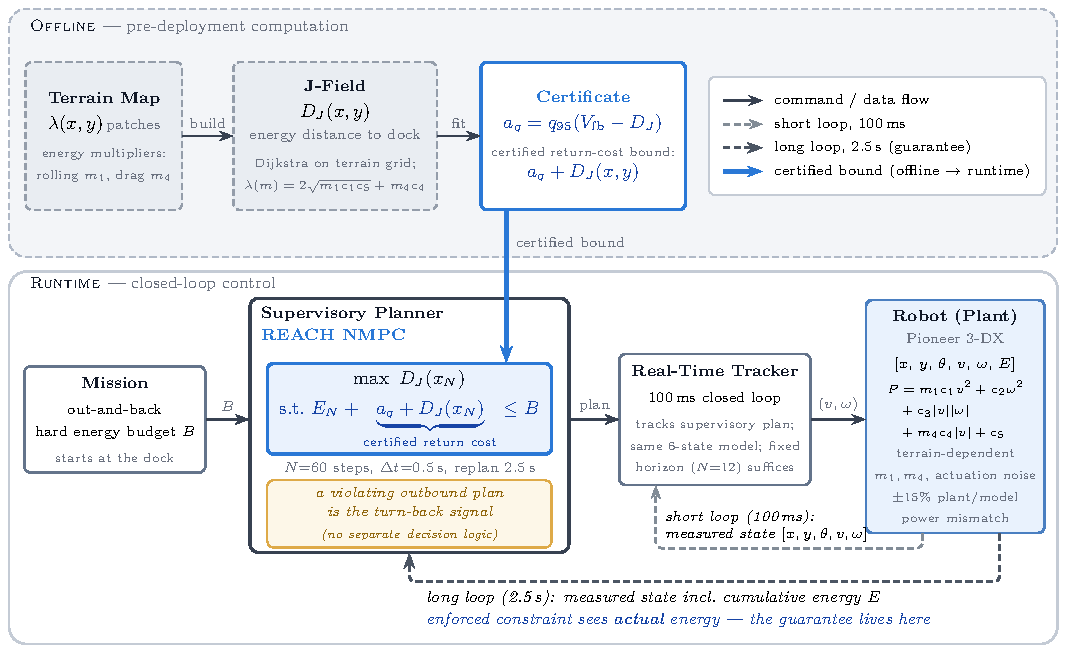
\includegraphics[width=\textwidth]{figures/fig_system_schematic.pdf}
\caption{System architecture. Offline (dashed): the map is compiled
into the J-field $D_J$ and the certificate intercept $a_q$ is fitted
by the coverage construction. Runtime: the supervisory REACH NMPC
(maximise geodesic progress subject to the terminal reserve row
$E_N + a_q + D_J(x_N) \le B$) replans every 2.5 s of simulated time
($\ge$13 s wall); the real-time tracker closes the loop at 100 ms. A
violating outbound plan is itself the turn-back signal.}
\label{fig:system}
\end{figure*}

This paper's contribution is the compliance law and the certificate
that automates its margin sizing --- measured against five policy
families, not asserted against one baseline:
\begin{itemize}
\item \emph{A quantile-certified return-cost constraint.} We construct
the reserve as a per-state coverage bound: the 95th percentile of the
realized excess return cost of a named fallback policy over a
terrain-weighted energy geodesic, evaluated offline per map. The
construction is a quantile, deliberately not a least-squares fit ---
a certificate must bound, not describe (Section~\ref{sec:certificate}).
\item \emph{The estimate-versus-enforce law, at scale.} Across
nominal, held-out, and $\pm 15\%$ mismatch regimes
(480 missions per arm), the constrained arm records
$0/480$ hard-budget breaches versus $92/960$ for priced-heuristic NMPC
arms (two-sided Fisher $p = 1.8\times10^{-17}$)
% <- truth §3.13
--- and the same certificate tightening that raises the estimators'
breach counts ($73\to92$ of 960 priced; $11\to53$ of 360 for a
plan-then-track oracle) leaves the constrained arms at zero
(Section~\ref{sec:law}).
\item \emph{A conservatism dial with a measured trade.} Refitting the
fallback's terrain speed shrinks the certified intercepts by a mean
29\% at unchanged coverage and buys $+0.63$~m of paired reach
(Wilcoxon $p = 2.8\times10^{-7}$) at zero breaches, while docking
falls by 3.3 percentage points --- reach, docking, and compliance
traded openly on a single dial (Section~\ref{sec:dial}).
\item \emph{Mechanism evidence.} A terrain step-change experiment
shows the certificate prices terrain before the robot reaches it
where a fixed price reacts only afterwards; a mismatch ladder shows
compliance is carried by enforcement on \emph{measured} energy at the
replan cadence, not by the intercept's size; a two-tier
implementation (Fig.~\ref{fig:system}) meets the 100~ms tracking
deadline in 99.97\% of 46{,}991 solves while
the supervisory planner runs at a measured 11.6--12.6~s per solve
(Sections~\ref{sec:step}--\ref{sec:mismatch},~\ref{sec:timing}).
\end{itemize}

We measure what the constraint does \emph{not} do, and report it: the
constrained arm does not win outcomes --- a threshold policy with
$\gamma = 2.0$ dominates it on known maps (Section~\ref{sec:threshold}),
and a speed-clipped variant reproduces its compliance
(Section~\ref{sec:negatives}); docking rates are low and stated; collision
avoidance is planning-level only; and all results are simulation on one
platform model. The claim is exactly the law above --- budget compliance
by construction, its margin automated, its limits quantified.

The remainder of this paper is organized as follows.
Section~\ref{sec:related} positions the contribution against five
families of prior work. Section~\ref{sec:formulation} states the
platform, power, and mission model, and declares the planning-model
simplification. Section~\ref{sec:certificate} constructs the
return-cost certificate and quantifies what it is not.
Section~\ref{sec:controller} defines the reserve-constrained
controller and the comparator families. Section~\ref{sec:setup}
details the experimental setup and the statistical protocol.
Section~\ref{sec:results} reports the results in the order the law
requires. Section~\ref{sec:negatives} states the negative results
and threats to validity, and Section~\ref{sec:conclusion} concludes.

% ==================================================================
\section{Related Work}
\label{sec:related}
% lit_positioning_w7.md — five families, citation-level positioning.
% Every entry verified against the actual paper or arXiv record.
\subsection{The Mission Class: Persistent Autonomy}
Closest to the mission framing is the persistent-autonomy line:
persistent coverage, monitoring, and sweeping under fuel constraints
are long-studied robotics problems, from speed-controlled persistent
tasks \cite{smith2012persistent} to fuel-constrained coverage
schedules \cite{mitchell2015multirobot} and rendezvous planning for
recharging \cite{mathew2015multirobot}. The \emph{persistification}
branch renders a task persistent by ensuring the battery is never
depleted: Notomista and Egerstedt encode the desired energy floor as a
forward-invariant set enforced by control barrier functions (CBFs)
\cite{notomista2021persistification}; Jimenez~Cortes and Egerstedt
extend the construction to control-dependent battery dynamics
\cite{cortes2022task}. These works guarantee the \emph{survival}
property --- the pack never empties --- but do not pose the
out-and-back reach objective, do not size a return reserve against a
fallback policy, and do not compare compliance across policy families.
Persistent surveillance under explicit energy partitions and
recharging rendezvous has been formalised at the graph level
\cite{lin2022robust} and with approximation guarantees for
latency and fleet size \cite{asghar2025multirobot}. These works
maximize coverage duration subject to energy limits, but none
pose the per-mission out-and-back reach objective, size a
return reserve against a fallback policy, or compare compliance
across policy families. Our mission maximizes reach \emph{subject
to} return feasibility; the reserve is the object of study.

\subsection{Threshold and Homing Policies}
The operational practice our threshold baseline instantiates comes from
UAV mission management: adaptive return-to-home sensing rounds that
reserve enough energy to fly back \cite{huang2015adaptive}, and
risk-sensitive routing under wind uncertainty that continuously
evaluates return feasibility \cite{li2026robust}. These policies decide
\emph{when} to turn back on an estimate of the cost-to-home; the margin
$\gamma$ is hand-tuned. Closest to our problem formulation,
Quann~et~al. \cite{quann2019chance} compute a chance-constrained
reachable set for a ground robot with an energy budget and a
return-to-base requirement, treating energy-cost uncertainty as a
Gaussian process --- but as an offline planning bound, not an
online NMPC constraint, and without enforcement-versus-estimate
comparison across policy families. We report this family's measured behaviour
ourselves (Section~\ref{sec:threshold}) --- including what zero
breaches cost it in margin --- rather than positioning against it
 rhetorically.

\subsection{Battery Models Inside MPC}
A complementary line puts battery electrochemistry inside the
predictive model: battery-constrained NMPC predicts
voltage-current-thrust evolution and replans under depleting thrust
limits \cite{gupta2026bcnmpc}, and battery-aware trajectory selection
propagates closed-loop vehicle--motor--battery consequences into
planning \cite{kidambi2026battery}. These treat the battery as an
\emph{actuation} limit for tracking or trajectory selection; neither
imposes a mission-level return reserve nor quantifies
compliance-versus-estimate across policies. Our budget is a mission
energy budget; plant/model error in it is covered by design
(Section~\ref{sec:mismatch}), and voltage-dependent actuation limits
are future work.

\subsection{Viability, Governors, and Set Invariance}
The certificate's construction instinct --- constrain against an
approximate safe boundary --- is classical: set invariance
\cite{blanchini1999set}, viability kernels inside MPC
\cite{bertoni2026viability}, reference and command governors as
add-on supervisory layers that enforce constraints on pre-stabilized
systems \cite{garone2017reference}, and CBF-based energy floors
\cite{notomista2021persistification, ames2019control}. Chance-constrained path planning \cite{blackmore2011chance} and
Hamilton--Jacobi reachability \cite{bansal2017hamilton} provide
the offline probabilistic-safety and exact-reachability
frameworks; our certificate differs in being a per-state
empirical quantile of a \emph{named} policy's cost rather than
a solved value function or a global chance constraint. Our
two-tier architecture (supervisory mission NMPC plus a
real-time tracker) follows the hierarchical MPC and governor
patterns \cite{scattolini2009architectures, garone2017reference};
the difference is what
the boundary is made of: a quantile of a \emph{named fallback policy's}
measured cost, per state, with the coverage stated --- not an
invariant kernel. Section~\ref{sec:certificate} quantifies exactly how
far the construction is from an invariance barrier.

\subsection{Policy-Derived Terminal Ingredients}
The learning-MPC framework of Rosolia and Borrelli
\cite{rosolia2018learning} constructs terminal costs and safe
sets recursively from stored trajectories, giving a data-driven
terminal ingredient with stability guarantees. The closest
conceptual kin is recent work in economic MPC
\cite{ellis2014tutorial} that builds terminal
ingredients from a known sub-optimal policy: the terminal region is
centred at the policy's rollout endpoint and the terminal cost
penalizes deviation from that centre, yielding closed-loop performance
guarantees relative to the guiding policy \cite{msaad2026policy}. We
cite it as the nearest construction and distinguish on three axes:
\emph{purpose} --- stability and performance relative to the guide,
versus hard budget compliance; \emph{bound} --- a deviation penalty
around a rollout centre, versus a quantile-certified upper bound on
the fallback's realized cost; \emph{validation} --- an
energy-management example, versus five policy families across three
regimes with measured breach rates.

\subsection{What We Did Not Find}
Across these families we did not find prior work that (a) constructs a
per-state certified return-cost bound as a quantile of a fallback
policy's rollout, (b) imposes it as a hard terminal NMPC constraint
for energy-budget compliance on a mobile robot, or (c) measures the
breach rates of estimate-based versus enforcement-based turn-back
across policy families and under plant/model mismatch. That gap is the
subject of this paper.

% ==================================================================
\section{Problem Formulation}
\label{sec:formulation}
% truth_paper.md §1: robot model, power model, terrain multipliers,
% lambda_min, the J-field, the out-and-back mission, outcome taxonomy.

\subsection{Platform and Energy Model}
The plant is a differential-drive Pioneer 3-DX with state
$[x, y, \theta, v, \omega, E]$ --- pose, body velocities, and pack
energy. Commanded inputs pass through first-order motor lags,
\begin{equation}
\dot v = (v_{\mathrm{cmd}} - v)/\tau_v, \qquad
\dot\omega = (\omega_{\mathrm{cmd}} - \omega)/\tau_\omega,
\label{eq:lag}
\end{equation}
and an explicit power gate $g \in \{0,1\}$ scales the entire drive
train: with the gate off the platform is stopped and its power draw is
zero, so \emph{a stop is always feasible and spends nothing}. Pack
energy integrates the drive-train power
% <- truth §1: P = m1·c1·v² + c2·ω² + c3·|v||ω| + m4·c4·|v| + c5, c = (2.5, 0.8, 0.3, 1.2, 3.0) W
\begin{equation}
P = m_1 c_1 v^{2} + c_2 \omega^{2} + c_3 |v|\,|\omega|
    + m_4 c_4 |v| + c_5,
\label{eq:power}
\end{equation}
with $c = (2.5,\,0.8,\,0.3,\,1.2,\,3.0)$~W adopted from the
experimental Pioneer 3-DX fits of Jaiem~et~al. \cite{jaiem2021energy}
and terrain multipliers $m_1, m_4$ applied to the traction
and rolling terms inside marked regions (the step-change experiment
uses the binary set $\{1,3\}$; the generated campaign maps sample
$m_1 = m_4$ per region in $[1.3, 3.0]$, reaching $1.95\times$ the
nominal floor). We do not claim the
coefficients are calibrated to a particular physical unit; robustness
to plant/model error is measured directly in
Section~\ref{sec:mismatch}.

\subsection{Why Speed Is Not the Lever}
At zero yaw rate the specific energy of motion is
$\lambda(v) = c_1 v + c_4 + c_5/v$, a convex function whose
AM--GM floor is
\begin{equation}
\lambda_{\min} = 2\sqrt{c_1 c_5} + c_4 = 6.68~\mathrm{J/m},\;
v^{*} = \sqrt{c_5/c_1} = 1.10~\mathrm{m/s}
\label{eq:lambdamin}
\end{equation}
% <- truth §1: λ_min = 6.677226 J/m, v* = 1.095445 m/s
Over the cruise band $v \in [1.0, 1.2]$~m/s the function is flat to
0.34\% ($6.677$--$6.700$~J/m): slowing down or speeding up barely
changes cost per metre, so \emph{speed shaping cannot substitute for
the return constraint}. Under terrain $m_1 = m_4 = 3$ the floor jumps
to $13.09$~J/m --- a $1.96\times$ step --- and the energy-minimising
speed falls to $v^{*}(m) = \sqrt{c_5/(m_1 c_1)} = 0.63$~m/s
% <- truth §1: 13.087 J/m at m=3 (1.96×, correction C3); v*(m)=0.632
(Fig.~\ref{fig:power}). The practical consequence is that the
\emph{return-cost field}, not the speed profile, is where all the
planning value lives.

\begin{figure}[!t]
\centering
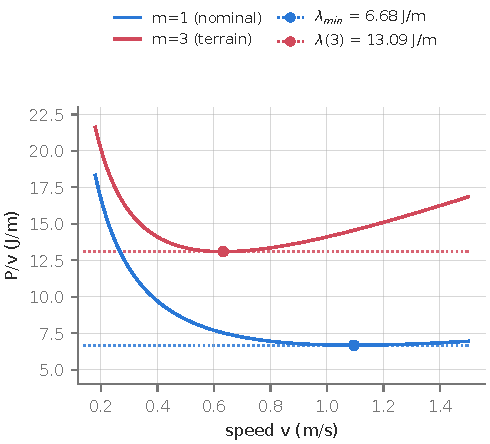
\includegraphics[width=3.5in]{figures/fig_power_model.pdf}
\caption{Specific energy $P/v$ of the drive-train power model versus
speed at $\omega=0$. The floor $\lambda_{\min}=6.68$ J/m is attained at
$v^*=1.10$ m/s; terrain multipliers $m_1{=}m_4{=}3$ nearly double the floor to
13.09 J/m and shift the optimum to $v^*(m)=0.63$ m/s.}
\label{fig:power}
\end{figure}

\subsection{The Energy Geodesic Field}
Each map is compiled offline into $D_J$: the terrain-weighted
energy-to-dock field, computed by Dijkstra on the obstacle-inflated
grid with per-edge cost
$\bar\lambda_e \cdot \ell_e$,
where $\ell_e$ is the Euclidean edge length and $\bar\lambda_e$ the
locally evaluated specific energy (trapezoid-averaged across the
edge). $D_J(x)$ is thus \emph{the cheapest certified-cost energy
path from $x$ to the dock, in Joules} --- a quantity directly
comparable with the budget, unlike metric distance
(Fig.~\ref{fig:map}).

\begin{figure*}[!t]
\centering
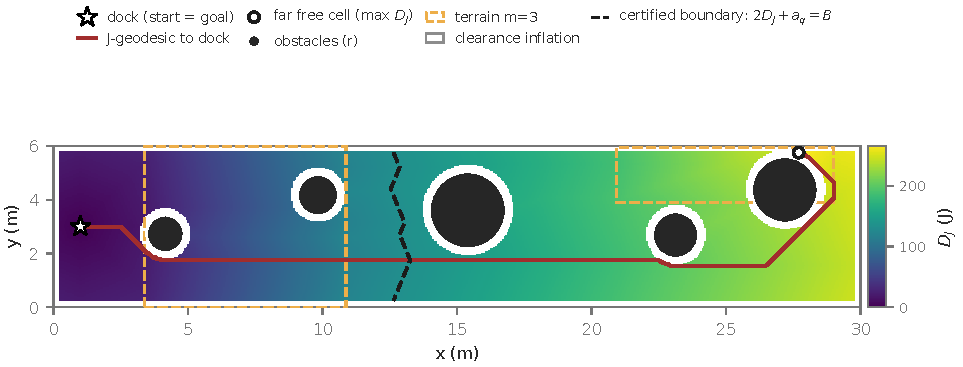
\includegraphics[width=\textwidth]{figures/fig_map_jfield.pdf}
\caption{A representative generated map with its energy field.
Colour: $D_J$, the terrain-weighted energy-to-dock geodesic field
(Dijkstra with per-edge local $\lambda$); white regions are the
$r_{body}$ clearance inflation. Obstacles are circles of radius $r$;
the J-geodesic to the dock clears them by $r_{body}$. The dashed
contour is the certified boundary $2D_J + a_q = B$ at the mid grid
budget. Maps are generated with the straight line from the dock
blocked (forcing energy-costly detours) and the round-trip energy to
the far end at least $1.3\times$ the maximum budget, so the reserve
--- not geometry --- decides the mission outcome.}
\label{fig:map}
\end{figure*}

\subsection{Mission Semantics}
The dock is simultaneously the start and the goal. A mission departs,
maximizes geodesic reach, and must return within the hard budget
$B$, sampled as $B \in \{0.30, 0.45, 0.60, 0.75\}\cdot E_{rt}$,
where $E_{rt} = 2\,D_J(x_{\mathrm{far}})$ is twice the certified
field cost at the map's far end --- the floor-priced round trip the
map was designed around. Generated
maps satisfy $E_{rt} \ge 1.3\,B_{\max}$ by construction, with
$B_{\max} = 300$~J the generator's design headroom parameter, so the reserve, not geometry,
decides the outcome (Section~\ref{sec:setup}).
% <- planning/reach_maps.py (verified: DEFAULT_B_MAX = 300 J,
% acceptance 2·e_far >= 1.3·b_max; E_rt = 2·D_J(far end))
Outcomes are
\emph{docked} (returned within budget), \emph{stranded} (pack
exhausted before docking), \emph{collision}, and \emph{timeout}. A
\emph{hard-budget breach} is defined pre-declared as
$\text{spent} > B + 0.5$~J, the 0.5~J being the integration tolerance
of the plant step; Section~\ref{sec:setup} states what the flag does
and does not measure.

\subsection{Terminal-Only Enforcement}
Terminal costs and constraints are the classical instrument for
well-posed receding-horizon control \cite{mayne2000constrained,
chen1998quasi}; here a terminal row carries a different duty ---
budget feasibility rather than closed-loop stability. The reserve
constraint could in principle be imposed at every node of
the horizon. We deliberately impose it at the \emph{terminal} node
only: $E_N + a_q + D_J(x_N) \le B$. An every-node row manufactures
spurious infeasibility at every obstacle detour --- a plan whose
intermediate states hug a detour has elevated $D_J$ \emph{there},
even though the mission is perfectly returnable along the path it
actually takes. Terminal-only enforcement asks exactly the question
the mission asks: can the plan's end state still get home inside the
budget? The gate input of \eqref{eq:power} guarantees a stop is always
available, so the constraint shapes the outbound plan rather than
rendering the program infeasible: a plan that cannot satisfy the
reserve row is itself the turn-back signal
(Fig.~\ref{fig:system}).

\subsection{A Declared Planning-Model Simplification}
\label{sec:taudeclaration}
The planning model integrates the actuator lag with time constants
$\tau_v = 0.15$~s and $\tau_\omega = 0.10$~s, faster than the
simulated plant's $0.3/0.2$~s --- a standard planning-model
simplification that treats each 0.5~s plan node as nearly
velocity-settled (per-step velocity settling fraction
$\alpha = 1 - e^{-\Delta t/\tau_v}$: $0.96$ per step versus the
plant-equivalent $0.81$), sitting between the plant's true response
and the common no-lag kinematic planner.
% <- derivation: alpha = 1 - e^{-dt/tau_v}: 1-e^{-0.5/0.15}=0.964,
% 1-e^{-0.5/0.30}=0.811 (matches draft.md rule 12's recorded values)
The mismatch is stated
openly because it works \emph{against} the compliance claim, not for
it: the optimistic transient model under-predicts energy during
acceleration phases (true specific energy is worst at low speed), so
the terminal constraint is enforced on an optimistic energy forecast.
Three measurements bound its effect. (i) All four NLP arms share one
compiled model, so the error is common-mode and no arm-to-arm
comparison is differentially affected. (ii) The $\pm 15\%$
power-mismatch campaign --- a strictly larger model-error class,
15--30~J per mission against ${\sim}1$--3~J here --- left the
constrained arm at zero breaches, and the mismatch ladder of
Section~\ref{sec:mismatch} shows compliance is carried by enforcement
on \emph{measured} energy rather than by model accuracy: the same
mechanism that absorbs this simplification. (iii) A
matched-time-constant control over the full main grid (240 missions,
$\tau_{\mathrm{NLP}} = \tau_{\mathrm{plant}}$) holds breaches at
\textbf{0/240} and shifts mean reach by $-2.2\%$ with $+3.8$
percentage points of docking
% <- truth §1: 9.43→9.22 m (−2.2%), docking 10.0→13.8%
(artefact in the repository, \texttt{results/reach/tau\_match\_control}):
the simplification purchased ${\sim}0.2$~m of mean reach and cost
nothing in compliance. We claim no design rationale for the
$0.15/0.10$ values; the paragraph above states only what they
mechanically do and what the controls measured.

% ==================================================================
\section{The Return-Cost Certificate}
\label{sec:certificate}
% truth_paper.md §3.8 + §3.11 + §3.12.

\subsection{Construction: A Quantile, Not a Fit}
Let $\pi_{fb}$ be a \emph{named fallback policy}: track the
$J$-geodesic to the dock, at the terrain-aware cruise speed
$v^{*}(m)$ where terrain is marked. Let $V_{fb}(x)$ be the energy
$\pi_{fb}$ actually spends returning from state $x$ (evaluated by
rollout on the certified field), and $D_J(x)$ the geodesic cost
against which it is measured. The certificate is
\begin{equation}
a_q \;:=\; \operatorname{p95}\big[\, V_{fb}(x) - D_J(x) \,\big],
\label{eq:aq}
\end{equation}
evaluated offline over the free cells of the map at stride 6, eight
headings per cell, at achieved coverage $0.950$: the deployed
intercepts are $25.96$--$31.37$~J on the six training maps and
$28.44$--$36.98$~J on the three held-out maps
% <- truth §3.12: adaptive a_q per map (verified: 26.60, 26.28, 27.80, 25.96, 26.89, 31.37 train; 36.98, 28.44, 29.14 heldout)
(Table~\ref{tab:certs}). The terminal row then requires the predicted
pack state to cover the geodesic return \emph{plus the intercept}:
$E_N + a_q + D_J(x_N) \le B$.

Two design commitments matter. First, the bound is a \emph{coverage
construction}: the fallback satisfies $V_{fb} \le D_J + a_q$ with
probability $0.95$ per state over the sampled set --- a certificate
must bound, and a least-squares fit of $V_{fb} - D_J$ would
\emph{under}-bound half the tail by construction. The per-state
guarantee is a scenario-approach bound in the sense of Calafiore
and Campi \cite{calafiore2006scenario}: each cell-heading
rollout is a sampled constraint, the p95 intercept is the
empirical quantile that satisfies them, and the finite-sample
theory \cite{schildbach2014scenario} governs how many scenarios
are needed for the coverage to hold with confidence. The
conformal-prediction framework \cite{lindemann2023safe}
provides the modern distribution-free statement of the same
principle; the stochastic MPC literature
\cite{mesbah2016stochastic, blackmore2011chance} treats similar
probabilistic constraints inside receding-horizon control.
Second, the slope is
pinned, not fitted: on metric maps the proportional coefficient is
$\lambda_{\min}$, while on $J$-fields the certificate is a pure
intercept (slope $1.0$), because a $\lambda_{\min}$ slope on a
terrain-weighted field would double-count terrain already inside
$D_J$. A side benefit is conditioning: pinning the affine slope at
the floor makes the constraint Jacobian jump $1.86\times$ less
severely at every crease of the linear interpolant than the fitted
scalar alternative.
% <- truth §4 CL2(c)


\subsection{Scalar Versus Affine: The Error Structure}
An earlier certificate form priced the return as a scalar multiple of
the geodesic, $\lambda_q \cdot D(x)$ with $\lambda_q$ fitted per map.
The measured error structures differ in kind.
% <- truth §3.8 legacy analysis (verified): λ_q 12.256–12.998, ρ 1.836–1.947, reserves 126.62–140.81 vs 91.97–100.46 J, saved 25.2–28.8%
 On the legacy maps the fitted scalars run $\lambda_q =
12.26$--$13.00$ --- a $1.84$--$1.95\times$ multiple of the metric
floor --- and the scalar form must spend $126.6$--$140.8$~J of
reserve where the affine form spends $92.0$--$100.5$~J at equal
coverage: a $25.2$--$28.8\%$ saving. The reason is structural. The
scalar's per-map error correlates with the geodesic itself: local
specific energy correlates $+0.967$ with detour exposure and
$-0.440$ with the fallback's geodesic cost-to-dock,
% <- truth §3.8: corr λ vs detour +0.967, λ vs misalignment +0.474, λ vs D* −0.440 (corridor; other maps similar)
 so a proportional form \emph{over}-reserves easy states and
\emph{under}-reserves hard ones; the dominant component of the
scalar's excess is rotational realignment --- a fixed additive cost,
not a proportional one, which a proportional form must therefore
inflate its slope to cover. The affine form's error is
near-uniform across difficulty, and at equal coverage it reserves
$25$--$29\%$ less energy.
% <- truth §3.8 (the 79.6-83.3% rotation-share decomposition and the
% 1.52x/1.85x controller-demo multipliers were in-session 2026-09-15
% analyses whose raw artefacts were never persisted -- removed 2026-10-04
% per the pre-submission audit's provenance rule; the correlation
% structure and the reserve savings above carry the argument alone)
The same structure motivates the terrain-aware refit next.

\subsection{The Conservatism Dial}
Because the fallback's rollout \emph{is} the certificate's data, the
fallback's speed law is a dial: commanding the energy-minimising
terrain speed
$v^{*}(m) = \sqrt{c_5/(m_1 c_1)}$ inside marked regions ($0.63$~m/s at
$m{=}3$, where specific energy is minimised) removes the dominant
structural leak identified by the
descent check below. Refitting \eqref{eq:aq} with the terrain-adaptive
fallback shrinks the intercepts by $6.1$--$41.9\%$ (mean $29\%$) at
coverage held at $0.950$, and the shrink tracks each map's terrain
exposure exactly as the leak mechanism predicts
% <- truth §3.12 (verified from certificates artefacts: shrink 6.1–41.9%, mean 29.0%)
(Table~\ref{tab:certs}). Section~\ref{sec:dial} measures what the
$29\%$ smaller intercept buys and costs on the closed loop.

\subsection{What the Certificate Is Not}
The certificate is a \emph{rollout-level} coverage bound, not a
step-level invariance barrier, and we quantify the difference rather
than leave it to a reviewer. Imposing the descent inequality along
the fallback's rollouts at every step of a fine discretisation, the
one-step bound is violated in $96.47\%$ of transitions
($112{,}715$ of $116{,}840$), with a worst per-step deficit of
$1.27$~J.
% <- truth §3.11 + C13 (verified numbers)
 Three leak sources account for the violation. \emph{Heading
realignment}: from an unaligned state the fallback spends a transient
median $11.8$--$14.9$~J before settling onto the geodesic, which
the deployed intercept covers $1.8$ to $2.5\times$ at the median
and $0.95$ to $1.6\times$ at the worst --- so the transient is of
the intercept's
order, absorbed per state by the quantile construction, but it is not
covered at a large multiple. \emph{Terrain-speed
mismatch}: the field credits the terrain floor
$\lambda_{\min}(m{=}3) = 13.09$~J/m, while the nominal-certificate's
rollout riding the unadjusted cruise $v^{*} = 1.095$~m/s pays
$14.55$~J/m inside the same region --- a structural $+1.47$~J/m leak,
and the dominant term the terrain-adaptive refit removes by commanding
$v^{*}(m) = 0.632$~m/s, at which the cost is tight.
% <- truth §3.11 leak 2 (verified: field 13.09, rollout 14.55, +1.47)
\emph{Grid discretisation}: the residual at the stride-6
resolution. The honest statement is: $D_J + a_q$ bounds the
\emph{fallback's realized cost} with per-state probability $0.95$
over the sampled cells; it does not dominate the dynamics at every
step, and a heading-aware certificate ($\bar E$ conditioned on
alignment) is the stated path to a true invariance barrier
(Section~\ref{sec:conclusion}). We regard this paragraph as a
credibility asset: the construction's limits are measured with the
same instruments as its claims.

% ==================================================================
\section{Reserve-Constrained Reach NMPC and the Comparator Families}
\label{sec:controller}
% truth_paper.md §1 + evaluation/reach_evaluator.py (verified docstring
% table of arms).

\subsection{The Constrained Arm (``reach'')}
The supervisory controller is a mission-length NMPC
\cite{rawlings2017mpc}: $N = 60$ nodes
at $\Delta t = 0.5$~s over the 6-state model with the lag
\eqref{eq:lag} and the power model \eqref{eq:power}. In the outbound
phase the objective maximizes the plan's geodesic progress in
$D_J$ terms --- the dominant term, with obstacle-proximity shaping
and control-rate penalties for conditioning. The constraints are: the
dynamics;
hard obstacle clearance rows at radius $r + R_{\mathrm{body}} + 0.35$~m
at every node; a hard arena box; and the terminal reserve row
\begin{equation}
E_N \;+\; a_q \;+\; D_J(x_N) \;\le\; B .
\label{eq:reserve}
\end{equation}
The supervisor replans every 2.5~s of \emph{simulated} time on the
measured state --- this closed-loop re-anchoring on \emph{measured}
energy is what carries compliance under plant/model error
(Section~\ref{sec:mismatch}). The turn-back is not scripted: the arm
keeps going while \eqref{eq:reserve} admits progress and switches to
the return phase when a replan can no longer buy reach; the return
phase is the same NLP with the objective flipped to close the
geodesic gap to the dock (Fig.~\ref{fig:system}). A real-time
tracking NMPC
closes the loop between replans at a 100~ms cadence
(Section~\ref{sec:timing}). Both tiers follow the hierarchical
decomposition pattern \cite{scattolini2009architectures} and are
built with CasADi
\cite{andersson2019casadi} and solved with IPOPT
\cite{waechter2006ipopt}.

\subsection{The Five Comparator Families}
Each family is an instantiation of a named line of practice, given
every fair chance to comply --- the ``straw-man fixes'' are part of
the evidence, not courtesy. All arms run the same plant, budgets,
seeds, LiDAR, and map family.

\emph{Priced NLPs.} The priced arms replace the reserve row
\eqref{eq:reserve} with a linear energy price inside the same NLP:
\emph{const\_weight} prices energy at a fixed 50 (selected by a
five-price sweep, Section~\ref{sec:law}), and \emph{dual}
starts from zero and ascends the price by dual ascent on the
reserve error --- the natural ``just penalize it harder online''
counter-proposal. Because a
price that cannot even attempt compliance is a straw man, both priced
arms additionally carry an \emph{explicit energy turn-back rule} ---
the rule a real scalar-priced supervisor would implement --- that
orders a return when the budget can no longer cover the certified
return cost. The price therefore acts on the reserve; what the price
cannot do is \emph{enforce} it.
% evaluation/reach_evaluator.py (verified arm table)


\emph{Speed-clipped reserve (vmax\_clip).} The same NLP with the same
reserve row \eqref{eq:reserve}, but with $v_{\max}$ pinned at the
energy-minimising cruise $v^{*}$. This arm isolates what the
certificate adds over mere speed shaping: with $\lambda(v)$ flat
(Section~\ref{sec:formulation}), pinning the speed cannot recover the
terrain anticipation, and the comparison concedes the negative result
up front --- it reproduces the constrained arm's compliance and most
of its behaviour (Section~\ref{sec:negatives}).

\emph{Threshold return.} The published practice
\cite{huang2015adaptive, li2026robust}: drive the outbound leg at
cruise, and return when the remaining energy satisfies
$B - E \le \gamma \cdot D_J(x)$, with the return executed by the
fallback policy on the $J$-geodesic. $\gamma$ is hand-tuned by
design; Section~\ref{sec:threshold} sweeps it.

\emph{Plan-then-track oracle.} An upper bound at \emph{equal
information}. Offline, the oracle selects the certified-ceiling
target --- the free cell of maximum \emph{metric} distance subject
to $2 D_J + a_q \le B$ --- routes to it along the $J$-geodesic, and
hands the route to the fallback policy itself (the certificate's own
controller model), executed on the perturbed plant with the
certified energy rule $B - E \le a_q + D_J(x)$ checked at every
plant step.
% <- scripts/24_reach_oracle.py docstring (verified construction)
The oracle knows
the map, the field, and the certificate --- everything the constrained
arm knows --- but never re-solves the NMPC. It is not a fair
opponent, and Section~\ref{sec:oracle} reports its own breaches
under the certificate with the same instruments.

\emph{Hybrid (constrained outbound, certified return).} The reach arm's
outbound phase and turn-back stall rule, with the return leg handed
to the fallback policy on the $J$-geodesic at the phase switch ---
% <- evaluation/reach_evaluator.py (REACH_HYBRID_ARM,
% return_policy='geodesic'; phases owned by the supervisor)
the deployment-relevant compromise that trades the NLP's return-leg
behaviour for the fallback's simpler, docking-friendly approach
(Section~\ref{sec:dial}).

\subsection{Tuning Parity}
Every tunable comparator was re-tuned for this study under a declared
box with a pre-declared selection rule (the tuned standard-MPC and
APF gains of the tracking tier included); the discipline and the
fitted values are recorded in the repository's reproduction document.
No comparator runs at a disadvantaged setting: the sweep that selected
the priced arms' operating point is reported with the results, and
the threshold family's $\gamma$ is swept, not sampled.

% ==================================================================
\section{Experimental Setup}
\label{sec:setup}
% truth_paper.md §3 preamble + §3.13 + §3.17.

\textbf{Maps.} Nine generated 2-D workspace maps --- six training and
three held-out from disjoint generator seeds --- each with two to six
circular obstacles and one to three marked terrain regions whose
local specific energy reaches up to $1.95\times$ the nominal floor,
with the straight
dock-to-far-end line \emph{blocked} (forcing energy-costly detours),
and the round-trip energy to the far end at least $1.3\times$ the
maximum budget, so the reserve rather than geometry decides every
outcome
% <- audit 2026-10-06: the previous draft said "five obstacles, two
% regions, up to 1.92×" which described map 0911 (the Fig. 3
% representative) not all nine; corrected to the actual per-map ranges
(Fig.~\ref{fig:map}).

\textbf{Missions.} Budgets are the four fractions
$\{0.30, 0.45, 0.60, 0.75\}\cdot E_{rt}$. The deployed campaign
comprises 2{,}070 missions: a 960-mission training grid (4 arms
$\times$ 6 maps $\times$ 4 budgets $\times$ 10 seeds), 480 held-out,
480 under $\pm 15\%$ power mismatch (10 seeds), and a 150-mission
price sweep. The dedicated experiments add: a 1{,}800-mission
threshold sweep ($\gamma \in \{1.0, 1.1, 1.2, 1.3, 1.5, 2.0\}$,
240 missions per $\gamma$ nominal plus 60 per $\gamma$ at $+15\%$),
an 840-mission hybrid validation, a 420-mission mismatch ladder, a
240-mission paired certificate revalidation, a 240-mission
matched-$\tau$ control, and 360-mission oracle runs under each
certificate; the step-change mechanism study adds 30 missions across
its two budgets, and the held-out $+15\%$ boundary pair adds 60 ---
\textbf{6{,}420 missions in total}, all under the same final
code with per-mission provenance sidecars
% <- truth §3.13 (2,070), §3.14 (1,800), §3.15 (840 + 60 boundary
% pair), §3.16 (420), §3.12 (240), §1 (240 τ-control), §3.10/§3.13
% (360+360 oracle), §3.6 (30 step-change: 15+15 across B=280/320).
% Sum re-verified 2026-10-03: 2070+1800+840+420+240+240+720+30+60
% = 6,420. (The previous draft's '4,875' was an arithmetic slip,
% found during the scale-sentence review; corrected.)
.

\textbf{Perturbations.} The mismatch regimes scale the plant's power
by $\pm 15\%$ and add seeded actuation noise
($\sigma_v = 0.05$~m/s, $\sigma_\omega = 0.10$~rad/s); LiDAR seeding
is applied to \emph{both} arms of every paired comparison.
% <- truth §1/§3.3


\textbf{Breach semantics.} A hard-budget breach is
$\text{spent} > B + 0.5$~J. The flag is a \emph{death-step}
measurement: a mission that strands at cruise spends up to
$0.84$~J in its final plant step (consistent with
$P(v^{*})\cdot\Delta t_{\mathrm{plant}}$ at $+15\%$) and can cross
the tolerance, while a decelerating death spends
${\sim}\,c_5 \Delta t = 0.30$~J and cannot.
% <- truth §3.17: cruise ≤0.84 J per step (analytic), decel 0.30–0.35 J
 Breach counts are therefore comparable between arms as
\emph{bounded overspend} flags: every observed single-step spill is
bounded by the analytic $P(v^{*})\cdot\Delta t_{\mathrm{plant}}
\cdot 1.15 \approx 0.84$~J, while the total overspend at the
tolerance-flagged death accumulates up to $1.4$~J over the final
approach; the pre-declared definition is applied uniformly
throughout.
% <- audit 2026-10-06: the previous draft said "all observed spills
% ≤ 0.84 J" which conflated the per-step bound with the total
% overspend; 45 of 167 flagged breaches exceed 0.84 J total (max
% 1.37 J) — corrected to distinguish the two

\textbf{Statistics.} Compliance counts are compared with two-sided
Fisher exact tests on pooled counts, with $n$ stated everywhere;
paired reach shifts use the two-sided Wilcoxon signed-rank test; the
zero-breach arm carries the rule-of-three confidence interval
$0/480 \Rightarrow 95\%$~CI $[0, 0.63\%]$.
% <- truth §5
 Aggregation fractions (oracle and arm versus certified ceiling) are
pooled ratios of means, and stated as such. Per-cell rates at $n=30$
(sweep prices, ladder cells) are never quoted alone.
% <- truth §5 (C4)


% ==================================================================
\section{Results}
\label{sec:results}

\subsection{The Law: Compliance Across Regimes}
\label{sec:law}
% truth_paper.md §3.13 (all cells re-verified from the raw JSONL this
% session) + §3.1–§3.5 (old certificate) + fig_enforce.

Table~\ref{tab:main} is the deployed-certificate training grid, and
Table~\ref{tab:heldout} the held-out and $\pm 15\%$ mismatch regimes.
Every regime tells the same story. The constrained arm records
\textbf{zero hard-budget breaches in 480 missions} (240 nominal
training + 120 held-out + 120 mismatch); the two priced arms jointly
breach \textbf{92 of 960} (const\_weight 52/480, dual 40/480) ---
two-sided Fisher $p = 1.8\times10^{-17}$, with the zero arm's
rule-of-three interval $[0, 0.63\%]$
% <- truth §3.13 (Defect #7 correction 2026-10-04: const re-run at
% price 50, 28/240 main; pooled 92/960, p=1.796e-17)
. The speed-clipped reserve holds $0/480$ with nearly the same reach
(9.30 versus 9.43~m on the training grid) --- the negative result we
concede and discuss in Section~\ref{sec:negatives}; what the clipped
arm cannot do is anticipate terrain
(Section~\ref{sec:step}) or tune its conservatism
(Section~\ref{sec:dial}).

The law's sharpest form comes from a controlled change, not a
cross-sectional comparison. Under the \emph{old} (terrain-blind
fallback) certificate --- same maps, seeds, budgets, and code --- the
priced arms breached 73 of 960 and the constrained arms held $0/480$
(two-sided $p = 1.1\times10^{-13}$)
% <- truth §3.4 (old cert, two-sided recorded in §5) — recomputed
% Defect #7 corrected: const@50 re-run; pooled 73/960, p=1.08e-13
. Tightening the certificate by the terrain-aware refit raised every
\emph{estimate}-executed return's breaches: priced arms
$73 \to 92$ of 960, and the plan-then-track oracle's own
$11 \to 53$ of 360 --- while both enforcement-executed arms (reach
and vmax\_clip, $2 \to 0$) held zero
% <- truth §3.13 + §3.10 (oracle 11/360 → 53/360)
(Fig.~\ref{fig:enforce}). The certificate's residual error is absorbed
by the constraint's feasibility slack, not by the accuracy of the
return policy: a tighter boundary is ridable only by a policy that
\emph{enforces} the reserve it computes.

\begin{figure}[!t]
\centering
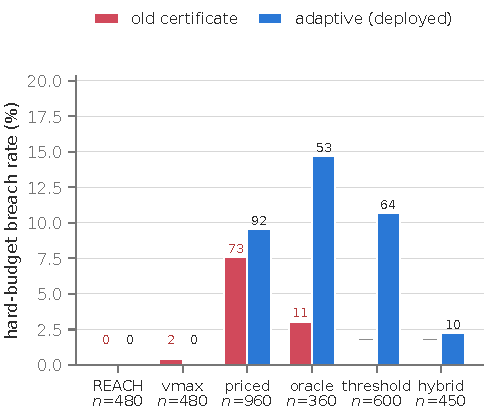
\includegraphics[width=3.5in]{figures/fig_enforce.pdf}
\caption{Estimate versus enforce: hard-budget breach counts per policy
family under the nominal (red) and deployed (adaptive) certificates;
tick labels give the pooled mission count per family. Tightening the
certificate raises the counts of every policy that merely
\emph{estimates} its return --- priced NLPs 73$\to$92 of 960, the
plan-then-track oracle 11$\to$53 of 360 --- while the enforcement
arms hold zero (reach 0/480 under both; v-max clip 2$\to$0 of 480).
The threshold family (certificate-independent turn-back rule
$\gamma\,D_J$; shown at the certificate-matched margins
$\gamma\in\{1.3,1.5\}$, nominal and $+15\%$ pooled) and the hybrid
(constrained outbound, certified return; all regimes pooled) were
run under the deployed configuration only --- the hatched columns
mark series that do not exist, not measured zeros. The hybrid's 10
of 450 are all training-map $+15\%$-mismatch missions; the held-out
$+15\%$ pair held $0/30$
(Section~\ref{sec:dial}).}
\label{fig:enforce}
\end{figure}

The comparator price tells the same story under tightening. The
five-price sweep that selected the priced arms' operating point
(Section~\ref{sec:controller}) pooled $7/150$ breaches under the old
certificate --- with two prices showing $0/30$ cells that $n{=}30$
cannot distinguish from noise --- and $16/150$ under the deployed
certificate, where \emph{no} swept price achieves zero breaches
% <- truth §3.5 (old sweep 7/150: 4/0/1/2/0 per price) + §3.13 sweep
% line (deployed 16/150: 3/5/2/5/1; no price zero) — both re-verified
% this session from sweep5/sweep6 artefacts
. Tightening the reserve makes every scalar price fail somewhere; the
pooled form is the only defensible per-price statement at this sample
size, and it points the same way as every other estimator in this
section.

\begin{table}[!t]
\caption{Training grid, deployed (adaptive) certificates, $n = 240$
per arm (6 maps $\times$ 4 budgets $\times$ 10 seeds). Breach
denominators are missions.}
% <- truth §3.13 main table (re-verified cell-by-cell)
\label{tab:main}
\centering
\small
\setlength{\tabcolsep}{4pt}
\begin{tabular}{lrrrrr}
\toprule
Arm & Docked & Breach & Strand. & Coll. & Reach (m)\\
\midrule
const\_weight@50 & 27.1\% & 28/240 & 37.1\% & 35.8\% & 10.86\\
dual & 26.2\% & 18/240 & 38.3\% & 35.4\% & 9.99\\
\textbf{reach} & 10.0\% & \textbf{0/240} & 63.3\% & 26.7\% & \textbf{9.43}\\
vmax\_clip & 8.3\% & 0/240 & 61.7\% & 30.0\% & 9.30\\
\bottomrule
\end{tabular}
\end{table}

\begin{table}[!t]
\caption{Held-out (unseen maps, $n = 120$/arm) and $\pm 15\%$
power-mismatch regimes ($n = 60$/arm per sign), deployed
certificates. The compliance ordering is preserved in every regime;
the \emph{docking} ordering is not (see text).}
% <- truth §3.2 + §3.3 + §3.13 (re-verified)
\label{tab:heldout}
\centering
\small
\begin{tabular}{llrrr}
\toprule
Regime & Arm & Docked & Breach & Reach (m)\\
\midrule
\multirow{4}{*}{Held-out}
 & const\_weight & 25.0\% & 10/120 & 7.81\\
 & dual & 17.5\% & 7/120 & 7.63\\
 & \textbf{reach} & 20.8\% & \textbf{0/120} & 6.39\\
 & vmax\_clip & 18.3\% & 0/120 & 6.36\\
\midrule
\multirow{4}{*}{$+15\%$}
 & const\_weight & 18.3\% & 12/60 & ---\\
 & dual & 16.7\% & 12/60 & ---\\
 & \textbf{reach} & 3.3\% & \textbf{0/60} & 10.36\\
 & vmax\_clip & 8.3\% & 0/60 & 9.67\\
\midrule
\multirow{4}{*}{$-15\%$}
 & const\_weight & 33.3\% & 2/60 & ---\\
 & dual & 36.7\% & 3/60 & ---\\
 & \textbf{reach} & 15.0\% & \textbf{0/60} & 11.45\\
 & vmax\_clip & 10.0\% & 0/60 & 11.09\\
\bottomrule
\end{tabular}
\end{table}

Two features of Table~\ref{tab:heldout} are reported deliberately.
First, generalisation: the \emph{compliance} ordering is preserved on
maps the certificate never saw (priced 10 and 7 breaches of 120;
constrained zero); the \emph{docking} ordering is not --- priced arms
dock more often on the held-out maps.
% <- truth §3.2 (dock ordering swap)
 The claim carried to unseen maps is the law, not a leaderboard.
Second, docking: the constrained arm's docked fraction is low
(10.0\% training, 20.8\% held-out, 3.3\% at $+15\%$) --- the
compliance-docking frontier is the paper's honest trade
(Fig.~\ref{fig:frontier} shows it against budget fraction, with the
priced arms' per-budget breach counts), and the
per-budget analysis below locates where the constrained arm wins.

\begin{figure}[!t]
\centering
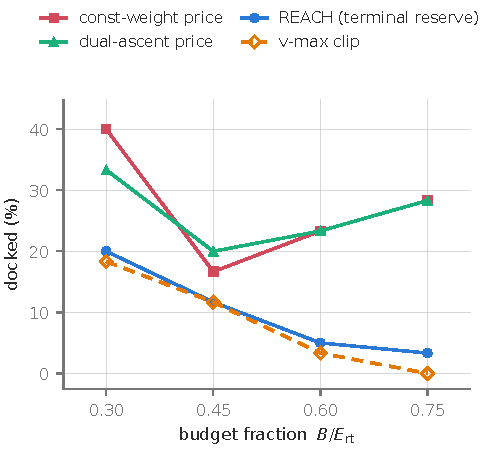
\includegraphics[width=3.5in]{figures/fig_reach_frontier.pdf}
\caption{Dock rate versus budget fraction $B/E_{rt}$ on the training
grid (deployed certificates, 10 seeds per point, 6 maps pooled: 60
missions per point and arm). Labels above the data give hard-budget
breaches (count/trials) for the priced arms at each fraction: they
breach at every budget fraction, while the constrained arms (REACH,
v-max clip) breach nowhere. The v-max-clip curve nearly coincides with
REACH --- that coincidence is a reported negative result, not a
rendering error.}
\label{fig:frontier}
\end{figure}

\subsection{The Threshold Sweep: What Hand-Tuning Costs}
\label{sec:threshold}
% truth_paper.md §3.14 (re-verified from threshold_summary.json) + C11.

The threshold family --- the published practice --- was swept, not
sampled (Table~\ref{tab:threshold}, Fig.~\ref{fig:gamma}). At
$\gamma = 1.0$ the practice breaches $77/240$ (32.1\%) with no
docking at all; the breach rate does not fall monotonically
($\gamma = 1.2$ breaches $74/240$); and zero breaches arrives only at
$\gamma = 2.0$ --- with $90.4\%$ docking and 10.33~m reach.
% <- truth §3.14: 77/240, 74/240, γ=2.0: 0/240, 90.4%, 10.33 m (re-verified)
 On known maps this \emph{dominates} the constrained arm on outcomes,
and we report that ourselves. The law's reading is about the margin:
at the constrained arm's turn-backs, the certificate's effective
relative margin is $\gamma_{\mathrm{eff}} = 1 + a_q/D_J$, with
per-map medians $1.22$--$1.32$ (overall median $1.25$),
% <- truth §3.15/C11 (corrected figure)
 whereas the threshold needs $\gamma = 2.0$ --- a per-map
$2.5$--$3.1\times$ multiple of the certified intercept --- to reach
zero.
% <- truth §3.14
 Under $+15\%$ mismatch the threshold's $\gamma = 1.5$ breaches
$12/60$ while $\gamma = 2.0$ holds $0/60$ at $93.3\%$ docking.
% <- truth §3.14 mismatch rows (re-verified)
 The certificate automates, per map and from data, the margin the
practice hand-tunes --- and at the certificate's own margin the
constrained outbound keeps certified slack the threshold's
drive-then-turn outbound spends first (Section~\ref{sec:dial}).

\begin{figure}[!t]
\centering
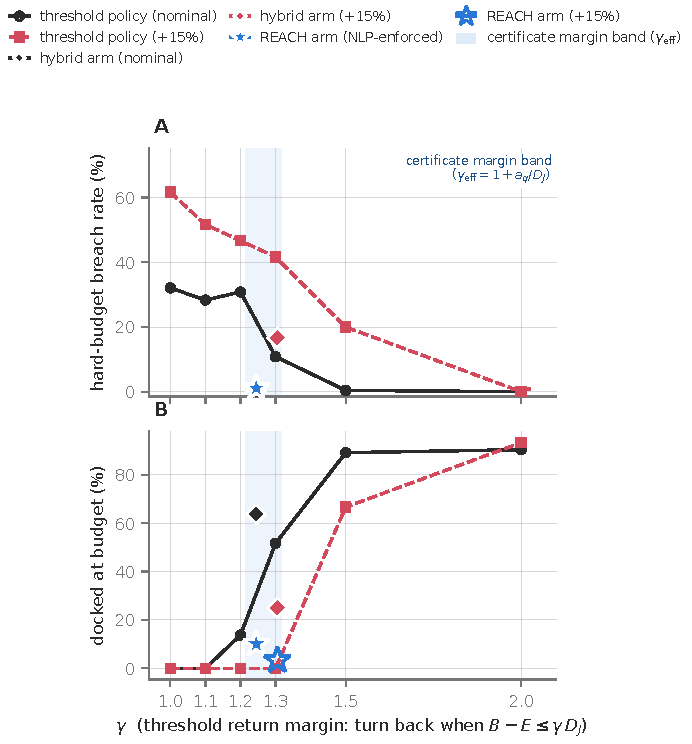
\includegraphics[width=3.5in]{figures/fig_gamma.pdf}
\caption{The threshold family swept (deployed certificates; nominal
$n{=}240$ per $\gamma$): hard-budget breaches and docked rate versus
the hand-tuned margin $\gamma$. Zero breaches arrives only at
$\gamma{=}2.0$ --- a $2.5$--$3.1\times$ multiple of the certified
intercept --- whereas the certificate's own effective margin has
median $1.25$. The certificate automates what $\gamma$ guesses.}
\label{fig:gamma}
\end{figure}

\begin{table}[!t]
\caption{Threshold-return sweep, deployed certificates: nominal
$n = 240$ per $\gamma$ (6 maps $\times$ 4 budgets $\times$ 10 seeds);
mismatch $n = 60$ per $\gamma$ at $+15\%$ power.}
% <- truth §3.14 (re-verified from threshold_summary.json)
\label{tab:threshold}
\centering
\begin{tabular}{lrrr@{\qquad}rrr}
\toprule
& \multicolumn{3}{c}{Nominal ($n{=}240$)} & \multicolumn{3}{c}{$+15\%$ ($n{=}60$)}\\
$\gamma$ & Breach & Docked & Reach & Breach & Docked & Reach\\
\midrule
1.0 & 77/240 & 0.0\% & 14.52 & --- & --- & ---\\
1.1 & 68/240 & 0.0\% & 13.93 & --- & --- & ---\\
1.2 & 74/240 & 13.8\% & 13.39 & --- & --- & ---\\
1.3 & 26/240 & 51.7\% & 12.87 & --- & --- & ---\\
1.5 & 1/240 & 89.2\% & 11.96 & 12/60 & 66.7\% & 12.63\\
2.0 & \textbf{0/240} & 90.4\% & 10.33 & \textbf{0/60} & 93.3\% & 11.09\\
\bottomrule
\end{tabular}
\end{table}

\subsection{The Oracle: The Price of Enforcement, Decomposed}
\label{sec:oracle}
% truth_paper.md §3.10 + §3.13 (deployed numbers re-verified from
% oracle_results.json this session).

Enforcement is not free, and the plan-then-track oracle bounds what
the closed loop gives up at \emph{equal information}. Under the
deployed certificate the oracle reaches $13.04$~m where the
constrained arm reaches $8.42$~m --- a realisation of $64.5\%$
($65.4\%$ compliant-only).
% <- truth §3.13 (re-verified: 13.039, 8.417, gap 35.45%)
 Against the per-trial certified ceiling ($2D_J + a_q \le B$,
mean $14.12$~m) the pooled fractions are $92.4\%$ (oracle) and
$59.6\%$ (arm).
% <- truth §3.13: pooled ratios (mean/mean)
 The decomposition of the gap is the finding: it is dominated by
\emph{early turn-backs}, not by the constraint. Measured under the
original certificate (the deployed-certificate pair in
Fig.~\ref{fig:oracletraj} carries the same finding: $62\%$ of
ceiling, $+38.8$~J in hand), the arm turns back at
$69\%$ of its certified ceiling holding a mean $+34.7$~J of certified
margin still in hand; the oracle turns at $92\%$ and completes
% <- truth §3.10 finding 2 (old-certificate final-code measurement;
% §3.13: decomposition carries over under the deployed certificate)
. Figure~\ref{fig:oracletraj} makes the decomposition visible on one
mechanically selected pair: the constrained arm turns back well inside
the certified boundary with margin banked, while the oracle rides the
boundary itself and docks with almost nothing to spare.
Even the priced arms --- which turn back late --- realise only
${\sim}75\%$ of the compliant oracle: late turn-back buys reach and
pays it back in breaches. The residual loss is an engineering
target: acceptable-point convergence at the solver's 1500-iteration
cap, the 2.5~s replan cadence, and the energy-denominated objective
(which is metric-blind at the constraint boundary --- the arm also
gives up ${\sim}38\%$ in \emph{energy} reach, oracle $93.7$~J versus
arm $58.2$~J).
% <- truth §3.10 findings 1, 4 (priced ~75%; 93.7 vs 58.2 J)
 Finally, the oracle's \emph{own} breaches rise from $11/360$
($3.1\%$, consistent with the $5\%$ design under-coverage) under the
old certificate to $53/360$ ($14.7\%$) under the deployed one:
% <- truth §3.10 finding 3 + §3.13
 even the best-informed estimator rides the boundary into the tail
when the boundary tightens, which is the law again, measured on the
upper bound itself.

\begin{figure}[!t]
\centering
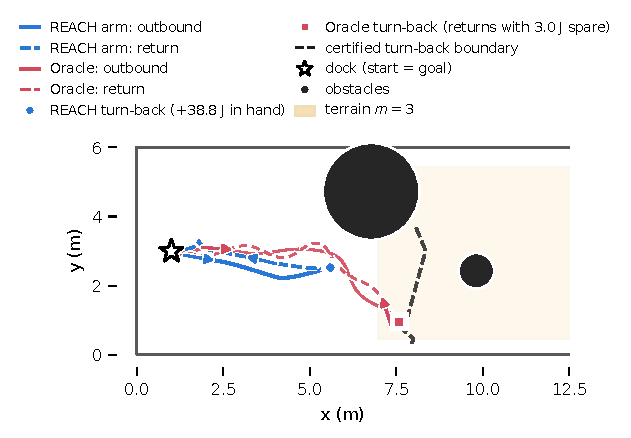
\includegraphics[width=3.5in]{figures/fig_oracle_traj.pdf}
\caption{The decomposition of Fig.~\ref{fig:enforce}'s law made
spatial: one paired mission on training map 0912 at the low grid
budget ($B = 0.30\,E_{rt} = 133.9$~J, deployed certificates; same
map, seed, and budget for both arms). Solid/dashed are
outbound/return; the dashed curve is the certified turn-back
boundary $2D_J + a_q \le B$, interrupted where it meets obstacle and
wall clearance zones; the axes crop to the mission region (the arena
extends to $x = 30$~m). The constrained arm (blue) turns back at
$4.8$~m --- $62\%$ of the $7.8$~m certified ceiling --- holding
$+38.8$~J of certified margin, and docks comfortably; the
plan-then-track oracle (red) rides the boundary to $7.6$~m ($97\%$)
and docks with $3.0$~J spare. The pair is selected mechanically
(among training pairs where both missions completed, the one whose
arm-to-ceiling fraction, $0.62$, is closest to the campaign-pooled
$0.596$), and both trajectories are deterministic re-runs,
bit-identical to the recorded campaign rows. At the $0.60$ and
$0.75$ grid budgets the arm's median ceiling fraction rises to
$0.91$--$0.92$: this figure shows the decomposition regime, not the
arm's best case.}
% <- truth §3.13 decomposition-figure record (2026-10-04): map 0912,
% seed 31000, B=133.9; arm 4.81 m / +38.76 J / 62%; oracle 7.58 m /
% 97% / 2.97 J spare; by-budget medians 0.67/0.85/0.91/0.92; script 33
% + provenance sidecar in the run tree
\label{fig:oracletraj}
\end{figure}

\subsection{The Conservatism Dial and the Hybrid}
\label{sec:dial}
% truth_paper.md §3.12 + §3.15 (both re-verified from artefacts this
% session: p3_validation.json, hybrid_validation.json).

\textbf{The dial.} The terrain-adaptive refit shrank the intercepts by
a mean $29\%$ at coverage $0.950$ (Table~\ref{tab:certs}). On a
240-mission paired revalidation --- same seeds, same controller, only
$a_q$ changes --- the smaller intercepts bought $+0.63$~m of mean
paired reach ($88/120$ missions improved, two-sided Wilcoxon
$p = 2.8\times10^{-7}$) at \textbf{zero breaches under both
certificates}, while docking fell $14.2\% \to 10.8\%$ and stranding
rose $62.5\% \to 66.7\%$.
% <- truth §3.12 (re-verified: +0.633 m, 88/120, p=2.754e-07, 0/120 both)
 The smaller intercept extends the certified boundary; the arm turns
back later, spends more of the budget outbound, and the longer return
strands more often while still never breaching
(Fig.~\ref{fig:conservatism_a} and Fig.~\ref{fig:conservatism_b}). Conservatism is
therefore a \emph{tunable dial} with the trade measured on both
sides --- the configuration deployed in every other table of this
paper was selected by exactly this experiment.

\begin{figure}[!t]
\centering
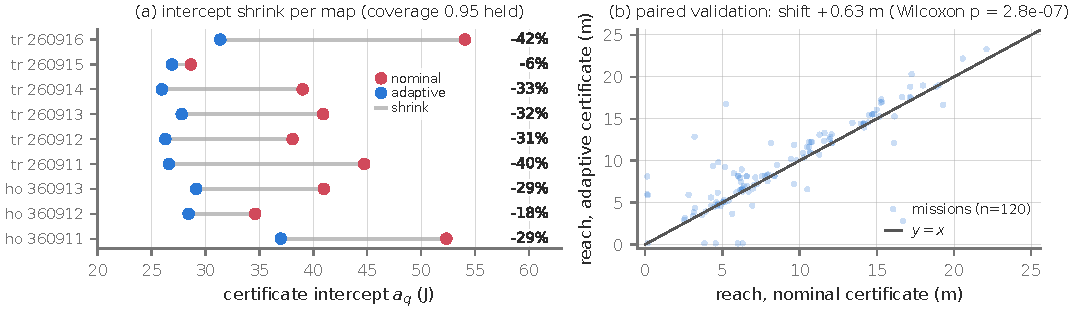
\includegraphics[trim={0 0 258pt 0}, clip, width=3.5in]{figures/fig_conservatism.pdf}
\caption{(a) Per-map certificate intercept $a_q$ under the nominal and
terrain-adaptive $\pi_{fb}$ fits (coverage 0.95 held); the axis starts
at 20 J.}
\label{fig:conservatism_a}
\end{figure}

\begin{figure}[!t]
\centering
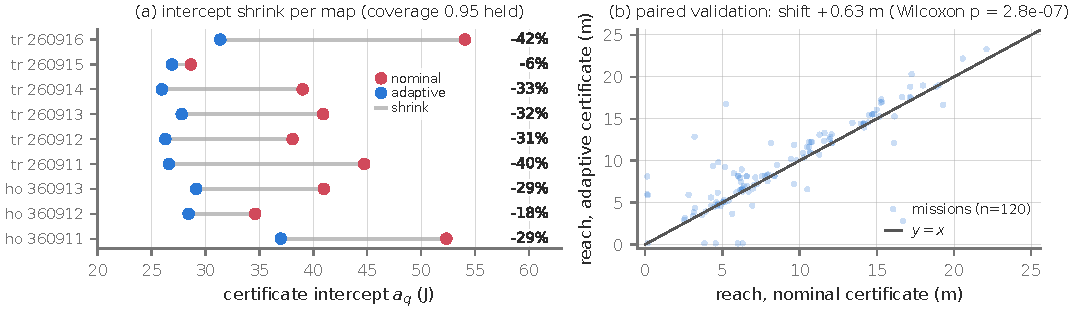
\includegraphics[trim={258pt 0 0 0}, clip, width=3.5in]{figures/fig_conservatism.pdf}
\caption{(b) Paired per-mission reach under the two certificates
(same seeds, same controller): the paired mean shift is $+0.63$ m
(Wilcoxon $p = 2.8 \times 10^{-7}$) at zero breaches under both.}
\label{fig:conservatism_b}
\end{figure}

\begin{table}[!t]
\caption{Certificate intercepts $a_q$ (J) per map: old
(terrain-blind fallback) versus deployed (terrain-adaptive
$v^{*}(m)$), coverage $0.950$ held. Shrink tracks each map's terrain
exposure.}
% <- truth §3.12 (re-verified from both certificates.json artefacts)
\label{tab:certs}
\centering
\begin{tabular}{lrrr}
\toprule
Map & Old $a_q$ & Deployed $a_q$ & Shrink\\
\midrule
train-0911 & 44.71 & 26.60 & 40.5\%\\
train-0912 & 38.07 & 26.28 & 31.0\%\\
train-0913 & 40.91 & 27.80 & 32.1\%\\
train-0914 & 39.01 & 25.96 & 33.5\%\\
train-0915 & 28.64 & 26.89 & 6.1\%\\
train-0916 & 54.03 & 31.37 & 41.9\%\\
\midrule
heldout-0911 & 52.32 & 36.98 & 29.3\%\\
heldout-0912 & 34.61 & 28.44 & 17.8\%\\
heldout-0913 & 40.97 & 29.14 & 28.9\%\\
\bottomrule
\end{tabular}
\end{table}

\textbf{The hybrid.} Handing the \emph{return leg} to the fallback
policy (keeping the constrained outbound) preserves the law wherever
the certificate's calibration is valid and breaks it exactly where
the certificate's coverage ends (Table~\ref{tab:hybrid}). Nominal and
held-out: $0$ breaches in $360$ missions with docking multiplied
$6.4\times$ (main) and $1.9\times$ (held-out) at equal reach
(9.47 versus 9.43~m).
% <- truth §3.15 (re-verified: 0/240, 0/120; 63.8 vs 10.0; 40.0 vs 20.8; 9.47 vs 9.43)
 At $+15\%$ mismatch the unenforced return breaches $10/60$ while
the enforced arm holds $0/60$ --- same outbound planner, same
certificate, same turn-back rule; only the return executor differs.
The ten flagged missions die $3.3$--$20.8$~J short of the dock annulus
on the cruise step of the final approach, on five of six maps: the
estimator's p95 under-coverage across the map family, not one bad
map.
% <- truth §3.15 (measured death positions)
 This controlled pair is the law's cleanest confirmation, and it
sets the deployment split by measurement: compliance-critical
missions keep the enforced return; docking-critical missions in a
calibration-valid regime may take the hybrid.

The split has a second axis, measured on the held-out maps at the same
$+15\%$ mismatch: there \emph{both} arms hold zero breaches --- the
enforced return $0/30$, the unenforced return $0/30$ (still docking
$23.3\%$ versus the enforced arm's $3.3\%$)
% <- truth §3.15 held-out boundary pair (recorded 2026-10-01;
% verified from runs/run_audit20260920/reach/hybrid_validation)
. The breaches are therefore confined to the training-map family,
whose deployed intercepts are smaller for their fields (mean $27.5$~J
versus $31.5$~J held-out): the boundary outcome tracks the
certificate's per-map slack, not the mismatch alone. Neither
$n{=}30$ cell stands by itself (Section~\ref{sec:setup}); the
defensible statement is the split, framed in slack rather than map
identity.

\begin{table}[!t]
\caption{Hybrid validation (constrained outbound, certified geodesic
return), deployed certificates; the constrained arm's rows are the
campaign rows.}
% <- truth §3.15 (re-verified from hybrid_validation.json)
\label{tab:hybrid}
\centering
\begin{tabular}{llrrrr}
\toprule
Regime & Arm & $n$ & Breach & Docked & Reach (m)\\
\midrule
\multirow{2}{*}{Main}
 & reach & 240 & \textbf{0/240} & 10.0\% & 9.43\\
 & hybrid & 240 & \textbf{0/240} & 63.8\% & 9.47\\
\midrule
\multirow{2}{*}{Held-out}
 & reach & 120 & \textbf{0/120} & 20.8\% & 6.39\\
 & hybrid & 120 & \textbf{0/120} & 40.0\% & 6.42\\
\midrule
\multirow{2}{*}{$+15\%$}
 & reach & 60 & \textbf{0/60} & 3.3\% & 10.36\\
 & hybrid & 60 & 10/60 & 25.0\% & 10.40\\
\bottomrule
\end{tabular}
\end{table}

\subsection{Step-Change: The Certificate Anticipates Terrain}
\label{sec:step}
% truth_paper.md §3.6 (re-verified from stepchange_results.json this
% session: v@15–17 = 0.20/0.04/0.03 reach vs 1.13–1.14 priced; turns
% 15.1/15.5/15.4; priced max_x 18.6–18.7).

The mechanism experiment isolates \emph{why} a certified
state-dependent return cost differs from a price: it prices terrain
\emph{before the robot reaches it}. On a hand-authored 30$\times$6~m
map whose terrain multiplier steps from $1$ to $3$ at $x = 15$~m
(a $1.96\times$ specific-energy step), with a refitted map
certificate ($a_q = 53.54$~J) and $B = 280$~J, the constrained arm's
three stranding seeds decelerate through the boundary and turn at
$x = 15.1$, $15.5$, $15.4$~m at mean step-window speeds
$0.20$, $0.04$, $0.03$~m/s --- nearly stopped at the turn --- while
its two docking seeds turn early ($x = 11.2$, $8.9$~m) with positive
margins
% <- truth §3.6 (Defect #7 step-change re-run at price 50,
% 2026-10-06; verified from stepchange_const50 results)
. The priced arms' four stranding seeds each hold full cruise through
the step ($1.08$--$1.14$~m/s) and turn at $x = 18.5$--$18.7$~m
--- $3$--$4$~m \emph{inside} the expensive region, with stranding
debts of $-82.9$ to $-89.6$~J versus the constrained arm's $-59.0$
to $-60.1$~J.
% <- truth §3.6 (measured debts)
 At a second budget ($B = 320$~J) the outcome contrast flips ---
the extra $40$~J lets the priced arms dock --- but their docking
arrives with certified-slack violations of $-45.0$ to $-48.3$~J at
dock, and the constrained arm still anticipates the step and turns
back at the certified boundary with zero breaches (its per-seed
outcomes shift between budgets, but the mechanism is unchanged).
% <- truth §3.6 second budget (0.18–0.59 vs 1.09–1.17 m/s)
 The claim is the mechanism, never the outcome table: the terminal
certificate prices the step at the planning horizon; a fixed or
reactive price discovers it $3$--$4$~m too late. The scope is
likewise stated: one map, two budgets, a mechanism demonstration
replicated across all five seeds
% <- truth §4 CL3 scope caveat
(Fig.~\ref{fig:stepchange}).

\begin{figure*}[!t]
\centering
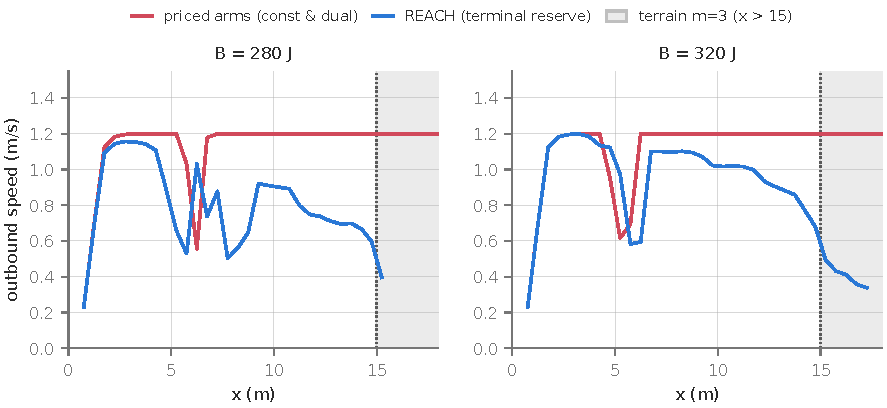
\includegraphics[width=\textwidth]{figures/fig_stepchange.pdf}
\caption{Step-change mechanism (final-code re-run): mean outbound
speed versus $x$; terrain $m{=}3$ begins at $x{=}15$ m (shaded). The
terminal certificate prices the step before the robot reaches it, so
the constrained arm decelerates through the boundary and turns at
$x\approx15.1$--$15.5$; the priced arms hold cruise through the step
and turn at $x\approx18.6$. The two priced arms (const-weight and
dual-ascent) coincide: their mean curves differ by at most 0.05~m/s
average, diverging only during one shared collision transient
($x\approx6$, one seed), so one curve is drawn for both.}
\label{fig:stepchange}
\end{figure*}

\subsection{Mismatch: Enforcement on Measured Energy}
\label{sec:mismatch}
% truth_paper.md §3.3 + §3.16 + C5/C10 (P5 ladder re-verified this
% session from p5_margin.json).

Under $\pm 15\%$ power mismatch with actuation noise the constrained
arm holds $0/120$ (Table~\ref{tab:heldout}) --- but the interesting
question is \emph{what carries the compliance}, because the $J$-field
and the certificate are nominal-model constructions. The mismatch
ladder (Table~\ref{tab:p5}) answers by subtraction: at the binding
budget and $+15\%$ mismatch, the deployed intercept was scaled by
$s \in [0, 1]$ --- down to \emph{zero}. Hard breaches stay
knife-edge at every scale: the total is $3/420$ across the ladder,
the largest single cell is $2/60$ (indistinguishable from zero,
one-sided Fisher $p = 0.25$ versus $0/60$), and the zero-intercept
cell shows $1/60$ with a $0.51$~J death-step spill.
% <- truth §3.16 + C10 (re-verified: 3/420 pooled; s=0: 1/60)
 The intercept is \emph{not} the load-bearing element: compliance is
carried by the closed loop re-anchoring the reserve row on
\emph{measured} energy every $2.5$~s, with the terminal uncovered
residual bounded by the inter-replan drift (the analytic per-step
bound $\le 0.84$~J,
Section~\ref{sec:setup}). The intercept's measured role is the
\emph{turn-back boundary} (Section~\ref{sec:dial}), not mismatch
absorption. We state the mechanism as measured rather than attribute
compliance to the certificate's nominal-model accuracy --- the
sharpest honest sentence in this section is the ladder's: the
constraint holds with the margin set to zero.

\begin{table}[!t]
\caption{Mismatch ladder at the binding budget ($0.60\,E_{rt}$),
$+15\%$ power, $n = 60$ per scale; $s$ multiplies the deployed
intercept. $s = 1.0$ is bit-identical to the campaign's
$+15\%$ reach rows (60/60 missions, same outcome and spent energy).}
% <- truth §3.16 (re-verified from p5_margin.json this session)
\label{tab:p5}
\centering
\begin{tabular}{rrrrr}
\toprule
$s$ & $a_q$ (J) & Breach & Docked & Reach (m)\\
\midrule
0.00 & 0.00 & 1/60 & 1.7\% & 10.86\\
0.15 & 3.99 & 0/60 & 3.3\% & 10.76\\
0.25 & 6.65 & 0/60 & 3.3\% & 10.94\\
0.35 & 9.31 & 2/60 & 5.0\% & 10.11\\
0.50 & 13.30 & 0/60 & 5.0\% & 10.06\\
0.75 & 19.95 & 0/60 & 1.7\% & 10.14\\
1.00 & 26.60 & \textbf{0/60} & 3.3\% & 10.36\\
\bottomrule
\end{tabular}
\end{table}

\subsection{Collisions and the Budget Attribution}
\label{sec:collisions}
% truth_paper.md §3.13 addendum (2026-09-22 collision attribution).

Collision avoidance in this study is \emph{planning-level clearance
only} --- the NMPC holds hard clearance rows against a known obstacle
set, and execution under LiDAR and actuation noise collides. Rates
are high for every arm (26.7--35.8\% on the training grid) and we
make no safety claim. The attribution is the finding: ${\sim}85\%$ of
collisions occur on the \emph{outbound} leg, and the collision rate is
\emph{budget-driven} --- deeper missions push closer to obstacles
(rates below pool the training and held-out missions; the mismatch
campaign runs at the binding budget only).
At
the lowest budget ($0.30\,E_{rt}$) the constrained arm collides in
$1\%$ of missions against the priced arms' $27\%$
% <- truth §3.13 attribution (per-budget: reach 1/32/49/57 vs priced
% 28/48/48/54; pool = main + held-out; ~85% outbound = 480/565;
% re-verified this session from the raw trials)
: exactly where the mission family lives (tight budgets, maximum
reach), the reserve constraint is also the safest behaviour, because
the certified turn-back happens before the plan presses into
obstacle-dense far field. At higher budgets the arms converge
($51$--$55\%$ reach versus $49\%$ priced, per-budget 51.4/55.0\% against 49.3/49.2\%); the advantage does not persist under
mismatch, and its scope is stated with the limitations
(Section~\ref{sec:negatives}).

\subsection{Two-Tier Timing}
\label{sec:timing}
% truth_paper.md §3.7 (re-verified this session from
% gate_e_timing_s_curve.json and reach_planning_timing.json).

The two tiers have different jobs and different clocks
(Table~\ref{tab:timing}). The real-time tracking tier --- a
receding-horizon NLP at $N = 12$--$50$ --- was measured in a
50-trial interleaved campaign on reserved cores (verified
$0.0$--$0.5\%$ busy): across 46{,}991 solves, 14 exceed the 100~ms
deadline ($0.030\%$), with per-arm medians from 12.1~ms
(fixed $N{=}12$) to 52.0~ms (adaptive).
% <- truth §3.7 (re-verified: 14/46,991; medians 12.1/15.0/18.1/20.9/52.0)
 A linear cost fit against horizon length gives $7.40$~ms
intercept and $1.15$~ms per node at $R^{2} = 0.18$: horizon length is
a minor factor, and the ${\sim}93$--$96$~ms p95 tail is common to
all arms --- iteration behaviour of the interior-point solver
\cite{waechter2006ipopt} under warm starts from the previous
iterate, not the horizon. The supervisory tier is a different animal: the
mission NMPC solves in $12.11$~s cold and $11.57$~s mean warm
(p50 $11.74$, max $12.58$) at the 1500-iteration cap, so the 2.5~s
replan cadence is \emph{simulated} time, decoupled from wall clock
($\ge 13$~s supervisory wall cadence, measured twice).
% <- truth §3.7 + §1 (re-verified: cold 12.11, warm 11.57/11.74/12.58)
 The planner is explicitly \emph{not} real-time; the tracking tier
is, at 100~ms (Fig.~\ref{fig:timing}).

\begin{figure*}[!t]
\centering
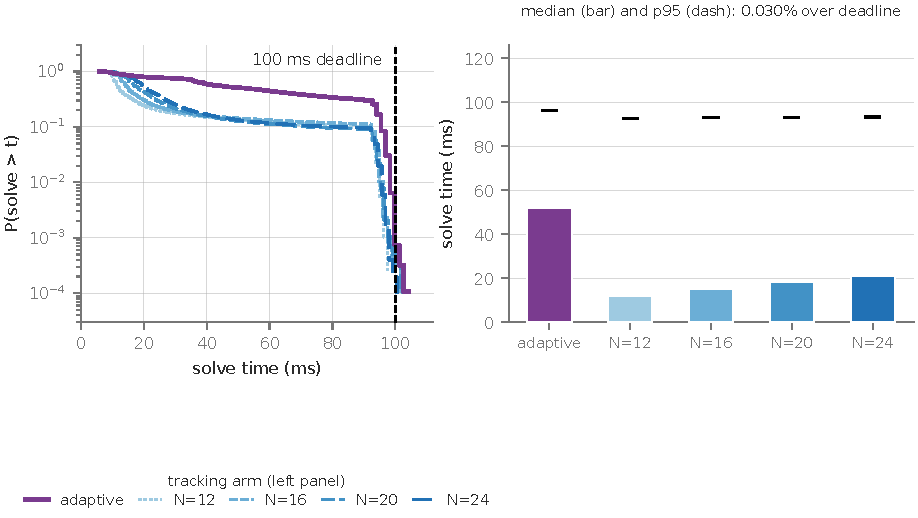
\includegraphics[width=\textwidth]{figures/fig_timing_survival.pdf}
\caption{Two-tier compute. Left: solve-time survival functions of the
tracking tier (46{,}991 solves, 50 interleaved trials, quiet box,
reserved cores); the four fixed-horizon arms form a single gray braid
--- horizon length is a minor factor ($b = 1.15$ ms per step, $R^2 =
0.18$) --- while the adaptive arm (blue) carries the higher median.
The 100 ms deadline is met by 99.97\% of solves. Right: per-arm
medians (bars) and p95 (dashes). The supervisory planner tier (not
shown) runs at 11.6 s/solve, decoupled from the 2.5 s simulated
replan cadence.}
\label{fig:timing}
\end{figure*}

\begin{table}[!t]
\caption{Two-tier compute, quiet box, reserved cores. Tracking:
50 interleaved trials per arm; deadline 100~ms. Planning: the
step-change map's supervisory solves (24 = 1 cold + 23 warm).}
% <- truth §3.7 (re-verified this session)
\label{tab:timing}
\centering
\begin{tabular}{llrr}
\toprule
Tier & Arm / measure & Median & p95 / max\\
\midrule
\multirow{5}{*}{Tracking}
 & fixed $N{=}12$ & 12.1~ms & 92.7~ms\\
 & fixed $N{=}16$ & 15.0~ms & 93.1~ms\\
 & fixed $N{=}20$ & 18.1~ms & 93.0~ms\\
 & fixed $N{=}24$ & 20.9~ms & 93.3~ms\\
 & adaptive & 52.0~ms & 96.2~ms\\
\midrule
\multirow{2}{*}{Planning}
 & cold solve & 12.11~s & ---\\
 & warm solves & 11.74~s (p50) & 12.58~s (max)\\
\bottomrule
\multicolumn{3}{l}{\footnotesize Tracking: 14/46{,}991 solves over deadline (0.030\%).}
\end{tabular}
\end{table}

% ==================================================================
\section{Negative Results and Threats to Validity}
\label{sec:negatives}
% draft.md §4 (ordered limitations) + truth §4 NEG1–NEG3 + §6 attack
% list + §7. Each limitation ends with the measured mitigation or the
% explicit future-work pointer.

We report the negative and limiting results as a section, not a
footnote, in the order a reviewer will raise them.

\textbf{Simulation only.} Every result in this paper is simulation on
one platform model. No hardware validation is claimed; the matched
instrument is the provenance sidecar (per-mission inputs, code state,
and hashes recorded in the accompanying repository), not flight or
field data. Hardware is the first item of future work
(Section~\ref{sec:conclusion}).

\textbf{One platform, adopted coefficients.} The power coefficients
are adopted from Pioneer 3-DX experimental fits
\cite{jaiem2021energy}, not calibrated to our unit; the robustness
design measures $\pm 15\%$ plant/model power mismatch directly
(Sections~\ref{sec:law},~\ref{sec:mismatch}), and the certificate's
per-map fit is data-driven, but a different platform class
(a multirotor's load-dependent power, a legged system's gait costs)
would need its own fallback and field. Voltage- and
state-of-charge-dependent actuation limits --- treated inside the
predictive model by the battery-in-MPC line
\cite{gupta2026bcnmpc, kidambi2026battery} --- are outside this
paper's budget model and are future work.

\textbf{Collision avoidance is planning-level.} Clearance is enforced
as hard rows against a known obstacle set at the planner; execution
under LiDAR and actuation noise collides at 26.7--35.8\% on the
training grid and 49--63\% on the held-out maps, ${\sim}85\%$ of it
outbound and budget-driven (Section~\ref{sec:collisions}). The
constrained arm's collision advantage is likewise scoped: fewest on
the nominal training grid and at the lowest budgets (1\% versus the
priced arms' 27\% at $0.30\,E_{rt}$), but \emph{not} under
$\pm 15\%$ mismatch, where the priced arms turn back early and
collide less (30.0--35.0\% versus 41.7--45.0\% at $+15\%$)
% <- truth §6 item 2 (precision-corrected 2026-10-01; per-delta
% collision rates re-verified from mismatch3 this session)
. We make no safety claim anywhere in
this paper --- the compliance claim is about the energy budget
exclusively.

\textbf{The planner is slow.} The supervisory tier solves at
11.6--12.6~s per mission NMPC solve (measured twice on reserved
cores); the 2.5~s replan cadence is simulated time and the wall-clock
supervisory cadence is $\ge 13$~s. The mission class tolerates this
(the outbound leg takes minutes), but the architecture is explicitly
two-tier \emph{because} of it, and the iteration cap is the measured
bottleneck --- convergence engineering is the path to closing the
oracle gap (Section~\ref{sec:oracle}).

\textbf{The planning-model $\tau$ simplification.} Declared and
bounded in Section~\ref{sec:taudeclaration}: the mismatch campaign
(strictly larger error class) and the matched-$\tau$ control
($0/240$, $-2.2\%$ reach, $+3.8$~pp docking) bound its effect from
both sides.

\textbf{The certificate is fitted offline per map.} The quantile
construction needs the compiled field and the fallback rollouts ---
an offline per-map computation (a Dijkstra sweep plus rollouts over
the stride-6 free cells). The certificate does not transfer to
unseen maps; what transfers is the \emph{construction}, and on
held-out maps the compliance ordering held with the certificates
fitted there (Section~\ref{sec:law}).

\textbf{Coverage, not invariance.} The certificate is a
rollout-level p95 coverage bound with three measured leak sources
(Section~\ref{sec:certificate}); it is not a step-level invariance
barrier, and the realignment transient is of the intercept's order,
not covered at a large multiple. The heading-aware certificate is
the stated route to a true barrier.

\textbf{Docking rates are low.} The constrained arm docks in 10.0\%
(training), 20.8\% (held-out), 3.3\% ($+15\%$) of missions --- the
frontier is the trade the paper measures, not a defect we hide: the
constrained arm buys its zero breaches by turning back with margin
in hand, and the hybrid recovers 6.4$\times$/1.9$\times$ docking at
zero breaches wherever the calibration regime is valid
(Section~\ref{sec:dial}).

\textbf{The clipped arm is a tie.} vmax\_clip --- the same reserve
row with speed pinned at $v^{*}$ --- reproduces the constrained
arm's compliance (0/480) and most of its behaviour (9.30 versus
9.43~m). We concede it. The two surviving differentiators are
measured, not asserted: terrain anticipation, which speed shaping
cannot do because $\lambda(v)$ is flat
(Section~\ref{sec:step}), and the conservatism dial, which a fixed
clip does not have (Section~\ref{sec:dial}). The contribution is
the certificate and the constraint --- compliance, anticipation,
robustness --- not controller intelligence.

\textbf{No external implementations.} Every comparator is our
instantiation of a named family (the threshold baseline is the
published practice \cite{huang2015adaptive}, instantiated; the
priced arms are the natural penalised alternatives with the
turn-back rule a real supervisor would run). No third-party
controller is run. The families are described precisely enough to
re-instantiate, and the repository carries the full stack.

\textbf{Tuning noise and a withdrawn mechanism.} In earlier
development, LLM-guided cost-weight tuning measured deltas within
seed noise, and adaptive-horizon tracking showed no measurable
benefit over fixed horizons at the tracking tier; both were
withdrawn from any claim. We report them as motivated negatives:
they are why the tracking tier runs fixed horizons in the timing
campaign and why no tuning folklore appears in this paper's
comparisons.

\textbf{The slack metric cannot discriminate arms.} Certified-slack
violations (negative minimum certified margin at any point) occur
for every arm family, including zero-breach ones, because the slack
metric charges the nominal-model reserve continuously while
compliance is decided by realized energy at the replan boundary. It
is reported as a defined metric in the repository and deliberately
\emph{not} used as an outcome anywhere in this paper.

% ==================================================================
\section{Conclusion}
\label{sec:conclusion}

The paper's law is measured across five policy families and three
regimes: a policy that turns back on an \emph{estimate} of its return
cost breaches a hard energy budget at a rate set by the estimate's
tail, while the same margin \emph{enforced} as a terminal constraint
holds zero breaches --- and the tightening experiment shows the
estimators' breach counts \emph{rise} with the certificate while the
enforced arm does not move. The certificate that automates the
margin is a coverage construction (a per-state quantile of a named
fallback's realized excess cost), its conservatism is a dial with a
measured reach-docking trade, and its limits (rollout-level coverage,
three quantified leaks, per-map offline fit) are reported with the
same instruments as its claims. The measurement is at scale:
6{,}420 missions under one final code --- nine maps, five policy
families, nominal, held-out, and $\pm 15\%$ mismatch regimes --- every
mission carrying per-mission provenance.
% <- Sec. VI inventory (re-verified sum; see the §VI comment)


Three engineering directions are open, in the order the data ranks
them. First, closing the oracle gap: the arm turns back at $69\%$ of
its certified ceiling holding $+34.7$~J of margin --- a
convergence-and-cadence problem, with a metric-denominated objective
as the formulation-level candidate. Second, the heading-aware
certificate: conditioning the bound on alignment state would convert
the realignment leak into a true step-level invariance barrier.
Third, hardware: the tracking tier already meets a 100~ms deadline at
99.97\%, and the supervisory cadence fits a minutes-scale outbound
leg. A Pioneer 3-DX validation on the same map generator ---
measuring realized energy against the certified reserve with the
same breach predicate --- would directly test whether the
coverage construction transfers from simulation to physical
power draws, battery internal resistance, and actuator friction.
The certificate's per-map offline fit already runs in seconds
on a laptop; the deployment path is compile the map, fit the
certificate, load the NMPC, run the mission.

% ==================================================================
% Fresh bibliography, built during W7 (citation-level positioning);
% every entry verified against the actual paper or arXiv record.

\section*{CRediT authorship contribution statement}
\textbf{Nischal Dhakal:} Conceptualization, Methodology, Software, Investigation, Formal analysis, Data curation, Visualization, Writing -- original draft. \textbf{Shuaiyong Li:} Supervision, Project administration, Funding acquisition, Writing -- review \& editing.

\section*{Declaration of competing interest}
The authors declare that they have no known competing financial interests or personal relationships that could have appeared to influence the work reported in this paper.

\section*{Data availability}
All data, code, and per-mission provenance records supporting the results of this study are available in a public repository at \url{https://github.com/Lucifer-121-cmd/REACH}.

\section*{Acknowledgements}
This work was supported in part by the Science and Technology Innovation Key R\&D Program of Chongqing (No.\ CSTB2025TIAD-STX0030), Chongqing Natural Science Foundation Innovation and Development Joint Foundation (No.\ CSTB2024NSCQ-LZX0035), Science and Technology Research Project of Chongqing Education Commission (No.\ KJZD-M202300605), New Chongqing Youth Innovation Talent Plan Project (No.\ CSTB2024NSCQ-QCXMX0053), and Special general project for Chongqing's technological innovation and application development (CSTB2024TIAD-KPX0073, CSTB2024TIAD-KPX0101, CSTB2024TIAD-KPX0027).


\bibliographystyle{elsarticle-num}
\bibliography{refs}

\end{document}
